\documentclass[twocolumn]{article}
\usepackage[utf8]{inputenc}
\usepackage[linesnumbered,ruled,vlined]{algorithm2e} 
\title{Assignment 1 \\ \small Fit a polynomial model.}
\author{David Padilla \\ Ignacio Pastore Benaim}
\date{\today}   % You can use \date{\today}
\usepackage{biblatex}
\addbibresource{references.bib}
\usepackage{graphicx}
\usepackage{hyperref}
\usepackage{color}
\usepackage{booktabs}
\usepackage{amsmath}

% Hyphen penalty
\hyphenpenalty=10000
\exhyphenpenalty=10000
\sloppy

\begin{document}

\maketitle

\section{Introduction}

In this report, we present the results of the first assignment of the Machine Learning course. The assignment consists of fitting 
several regression models to a noisy dataset generated from a polynomial function. The figure \ref{fig:polynomial_data} shows 
the dataset which contains 500 data points. The majority of the methods seen in class were explored for the sake 
of completeness. A comparison of the results is presented along with the election of the optimal models. 

We explore multiple methods, including k-NN, linear regression variants, and regularized 
polynomial regressions. The optimal models were selected based on cross-validation, 
and final test results are reported. Finally, a short discussion and conclusion are presented.

The complete code used for this analysis can be found in a \href{https://colab.research.google.com/drive/1Gg35b8epwsI3nkCeiqCgBeFCd3aNdahI?usp=sharing}{Google Colab Notebook}.

\begin{figure}[!htb]
\centering
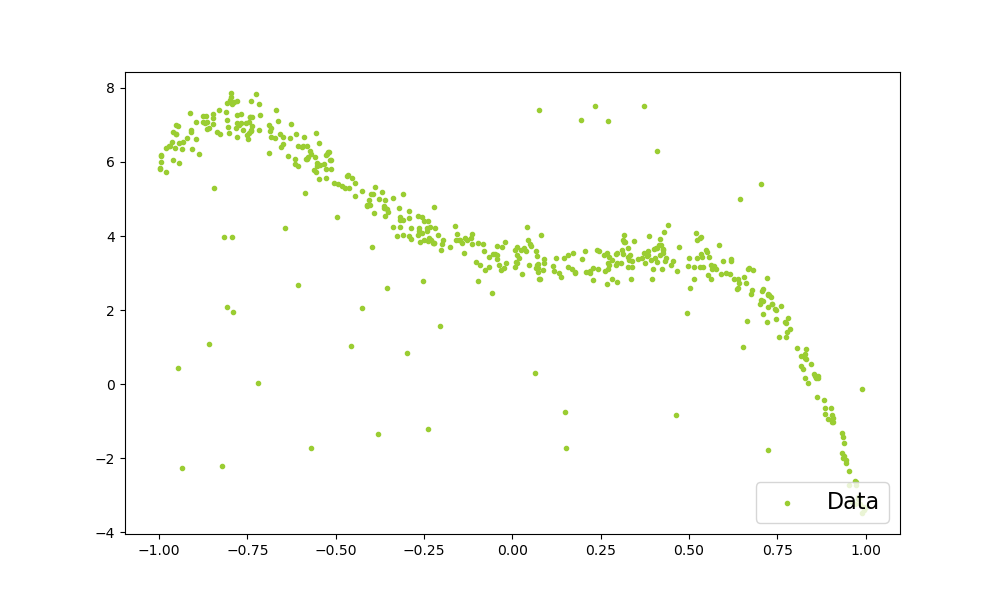
\includegraphics[width=0.95\columnwidth]{images/scatter_plot.png}
\caption{Polynomial function generated with random noise.}
\label{fig:polynomial_data}
\end{figure}
  
\section{Materials \& Methods}

The original dataset consists of 500 data points, which were split into training (81\%), 
validation (9\%), and test (10\%) sets. No outlier removal was performed. The evaluation process involved 3 key steps: 
initial screening with validation, cross-validation of selected models, and final evaluation on the test set.

All models were implemented in Python with the numpy, pandas and scikit-learn libraries.

\subsection{Initial Screening with Validation set}
Various models (described in Section \ref{sec:models}) were first evaluated using a validation set. 
The purpose of this step was to quickly assess model performance and identify promising candidates.

\subsection{Cross-Validation of Selected Models}
Based on the validation results, a subset of models was chosen for cross-validation with
\( k = 10 \) folds. The average performance across the folds was used to further narrow down the best-performing models.

\subsection{Final Testing on Test Set}
After cross-validation, the best models were retrained with the training and validation set combined. 
The evaluation was finally made on the test set.



\subsection{Models}\label{sec:models}

We tested several different models, including k-Nearest Neighbors (k-NN), 
various linear regression models, and polynomial regression with regularization.

\subsubsection{k-NN}
The k-NN model was implemented with an optimal \( k = 17\) obntained from a grid search with 5-fold cross-validation 
over the range of 1 to 20.

\subsubsection{Linear Regression Variants}
Despite knowing that a linear model might not be the outmost appropiated for this task, 3 variants were implemented
to compare with other methods:

\begin{itemize}
    \item Standard Linear Regression.
    \item Huber Regression.
    \item RANSAC Regression.
\end{itemize}

\subsubsection{Polynomial Regression with Regularization}
Polynomial regression models were fitted using Ridge and Lasso regularizations to 
control overfitting. We applied 5-fold cross-validation using a grid search over 
polynomial degrees from 1 to 12 and regularization strengths \(\lambda\) in the range of [0.01, 0.1, 1, 10, 100]
to find the optimal configurations. The initial results showed that the best-performing 
models were Ridge Regression with degree 12 and \(\lambda\) = 0.01 and 
Lasso Regression with degree 6 and \(\lambda\) = 0.01.

However, visual inspection suggested that high-degree polynomial models were prone to overfitting. To balance model complexity 
and performance, we decided to focus on polynomial degrees 6 and 7 for further analysis, 
both with and without regularization. 

\subsection{Evaluation Metrics}
Through all the phases, the models were evaluated using 2 primary metrics:
\begin{itemize}
    \item Mean Squared Error (MSE).
    \item \( R^2 \) Score.
\end{itemize}


\section{Results}

\subsection{Initial Validation Results}
The first screening of models was done using the validation set. Table \ref{tab:validation} shows the MSE and \( R^2 \) 
scores for the various models during the validation phase. Based on these results, linear models were discarded for further analysis.

\begin{table}
\centering
\caption{Initial validation performance}
\label{tab:validation}
\begin{tabular}{|l|l|c|c|}
\toprule
                           Model &   MSE &    R2 \\
\midrule
                      KNN (k=17) & 0.514 & 0.916 \\
                          Linear & 0.978 & 0.841 \\
                           Huber & 1.059 & 0.828 \\
                          RANSAC & 1.337 & 0.782 \\
           Polynomial (degree=6) & 0.425 & 0.931 \\
Ridge (degree=6, $\lambda=0.01$) & 0.430 & 0.930 \\
Lasso (degree=6, $\lambda=0.01$) & 0.474 & 0.923 \\
           Polynomial (degree=7) & 0.509 & 0.917 \\
Ridge (degree=7, $\lambda=0.01$) & 0.465 & 0.924 \\
Lasso (degree=7, $\lambda=0.01$) & 0.474 & 0.923 \\
\bottomrule
\end{tabular}
\end{table}


\subsection{Cross-Validation Results}
The cross-validation results are summarized in Table \ref{tab:cross_validation} showing the MSE and \( R^2 \) scores.
Based on these results all the models were retained for further analysis.

\begin{table}
\centering
\caption{Cross-validation performance}
\label{tab:cross_validation}
\begin{tabular}{|l|l|c|c|}
\toprule
                           Model &   MSE &    R2 \\
\midrule
           Polynomial (degree=6) & 1.770 & 0.682 \\
Ridge (degree=6, $\lambda=0.01$) & 1.769 & 0.682 \\
Lasso (degree=6, $\lambda=0.01$) & 1.813 & 0.676 \\
           Polynomial (degree=7) & 1.763 & 0.684 \\
Ridge (degree=7, $\lambda=0.01$) & 1.765 & 0.683 \\
Lasso (degree=7, $\lambda=0.01$) & 1.813 & 0.676 \\
                      KNN (k=17) & 1.803 & 0.705 \\
\bottomrule
\end{tabular}
\end{table}


\subsection{Test Set Results}
Finally, the selected models were tested on the test set. Table \ref{tab:tests} shows the final MSE and \( R^2 \) scores on the test set.

\begin{table}
\centering
\caption{Tests}
\label{tab:tests}
\begin{tabular}{|l|l|c|c|}
\toprule
                           Model &   MSE &    R2 \\
\midrule
                      KNN (k=17) & 1.127 & 0.807 \\
           Polynomial (degree=6) & 1.146 & 0.803 \\
Ridge (degree=6, $\lambda=0.01$) & 1.143 & 0.804 \\
\bottomrule
\end{tabular}
\end{table}


\section{Discussion}
The initial screening confirmed that linear models were unsuitable and were discarded as expected. 
Surprisingly, k-NN performed similarly to the more complex polynomial models. The MSE values ranged from 1.127 to 1.160, and when rounding up the  \( R^2 \)  scores, all models 
explained around $80\%$ of the variance in the data.

Ridge and Lasso regularizations showed no significant improvements, suggesting that 
overfitting was not an issue. Given the comparable results, we would choose between k-NN and polynomial regression for their simplicity. 
Future work could involve removing outliers to refine the results further.

\section{Conclusion}
All tested models—k-NN, polynomial regression, and regularized variants—showed comparable performance,
 explaining approximately $80\%$ of the variance in the data. Minor differences in the metrics indicate no clear 
 best model, making k-NN and polynomial regression preferable for their simplicity. Future work could focus on enhancing 
 model performance through data preprocessing techniques such as outlier removal.

\end{document}
